\label{app:evaluation-app}
To enable systematic clinician evaluation within the Trusted Research Environment, we developed a custom evaluation application using FastAPI (backend) and Next.js (frontend). The application ran locally within the TRE to ensure patient data never left the secure environment.

The interface was designed to support the hierarchical evaluation framework. In the first screen (Figure~\ref{fig:evaluation_apps}a), the clinician reviewed the structured patient data---seeing exactly what the System saw---and determined whether sufficient information existed to assess intervention necessity. \removed{This stage identified 23 cases excluded for data quality issues.} \added{This stage identified 8 of the 23 excluded cases (see Appendix~\ref{sec:case-sampling} for the full exclusion criteria and breakdown).} On the second screen (Figure~\ref{fig:evaluation_apps}b), the clinician reviewed both patient data and System analysis side-by-side, grading each identified issue as correct or incorrect, noting any missed issues, and assessing intervention appropriateness. \added{A further 11 exclusions were flagged at this screen after the clinician identified a suspected data error in the record; the remaining 4 reviews could not be completed due to limitations of the application.}

Results were saved locally to JSON files for subsequent analysis.

\begin{figure}[ht]
    \centering
    \begin{subfigure}[t]{0.48\textwidth}
        \centering
        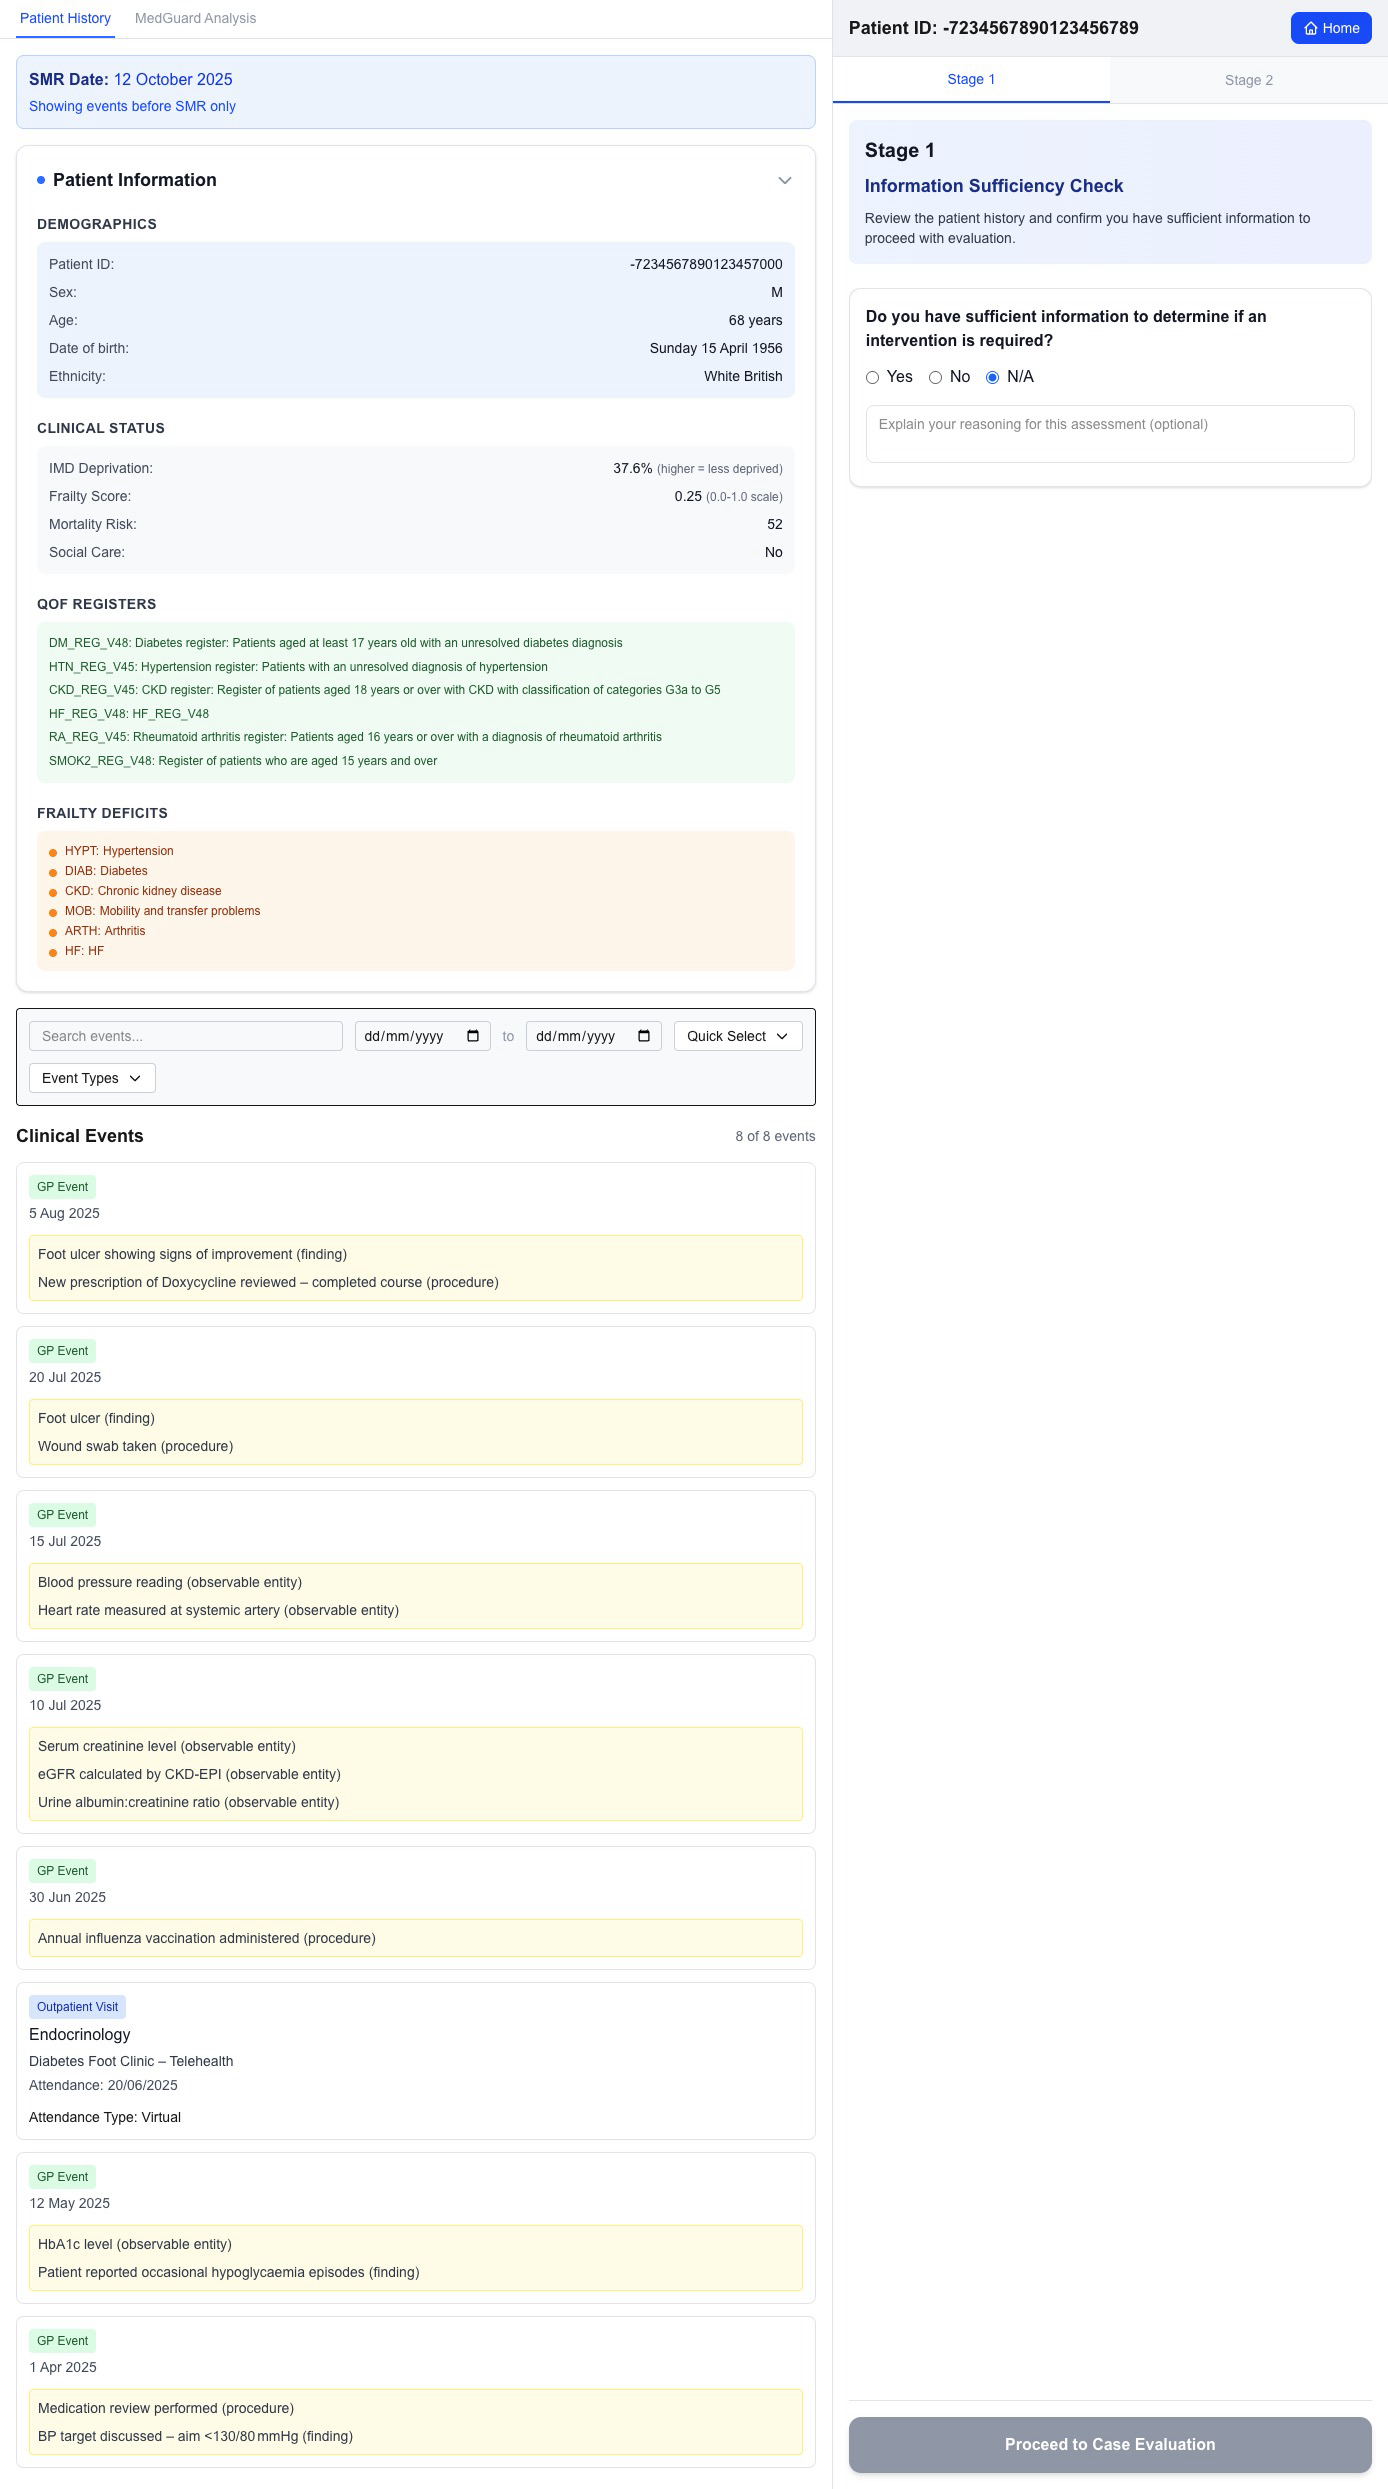
\includegraphics[width=\textwidth]{figures/stage_1_evaluation_app.png}
        \caption{Screen 1: The clinician can look at the structured patient data and decides whether they have sufficient information to determine if an intervention is required for this patient.}
        \label{fig:stage_1_evaluation_app}
    \end{subfigure}
    \hfill
    \begin{subfigure}[t]{0.48\textwidth}
        \centering
        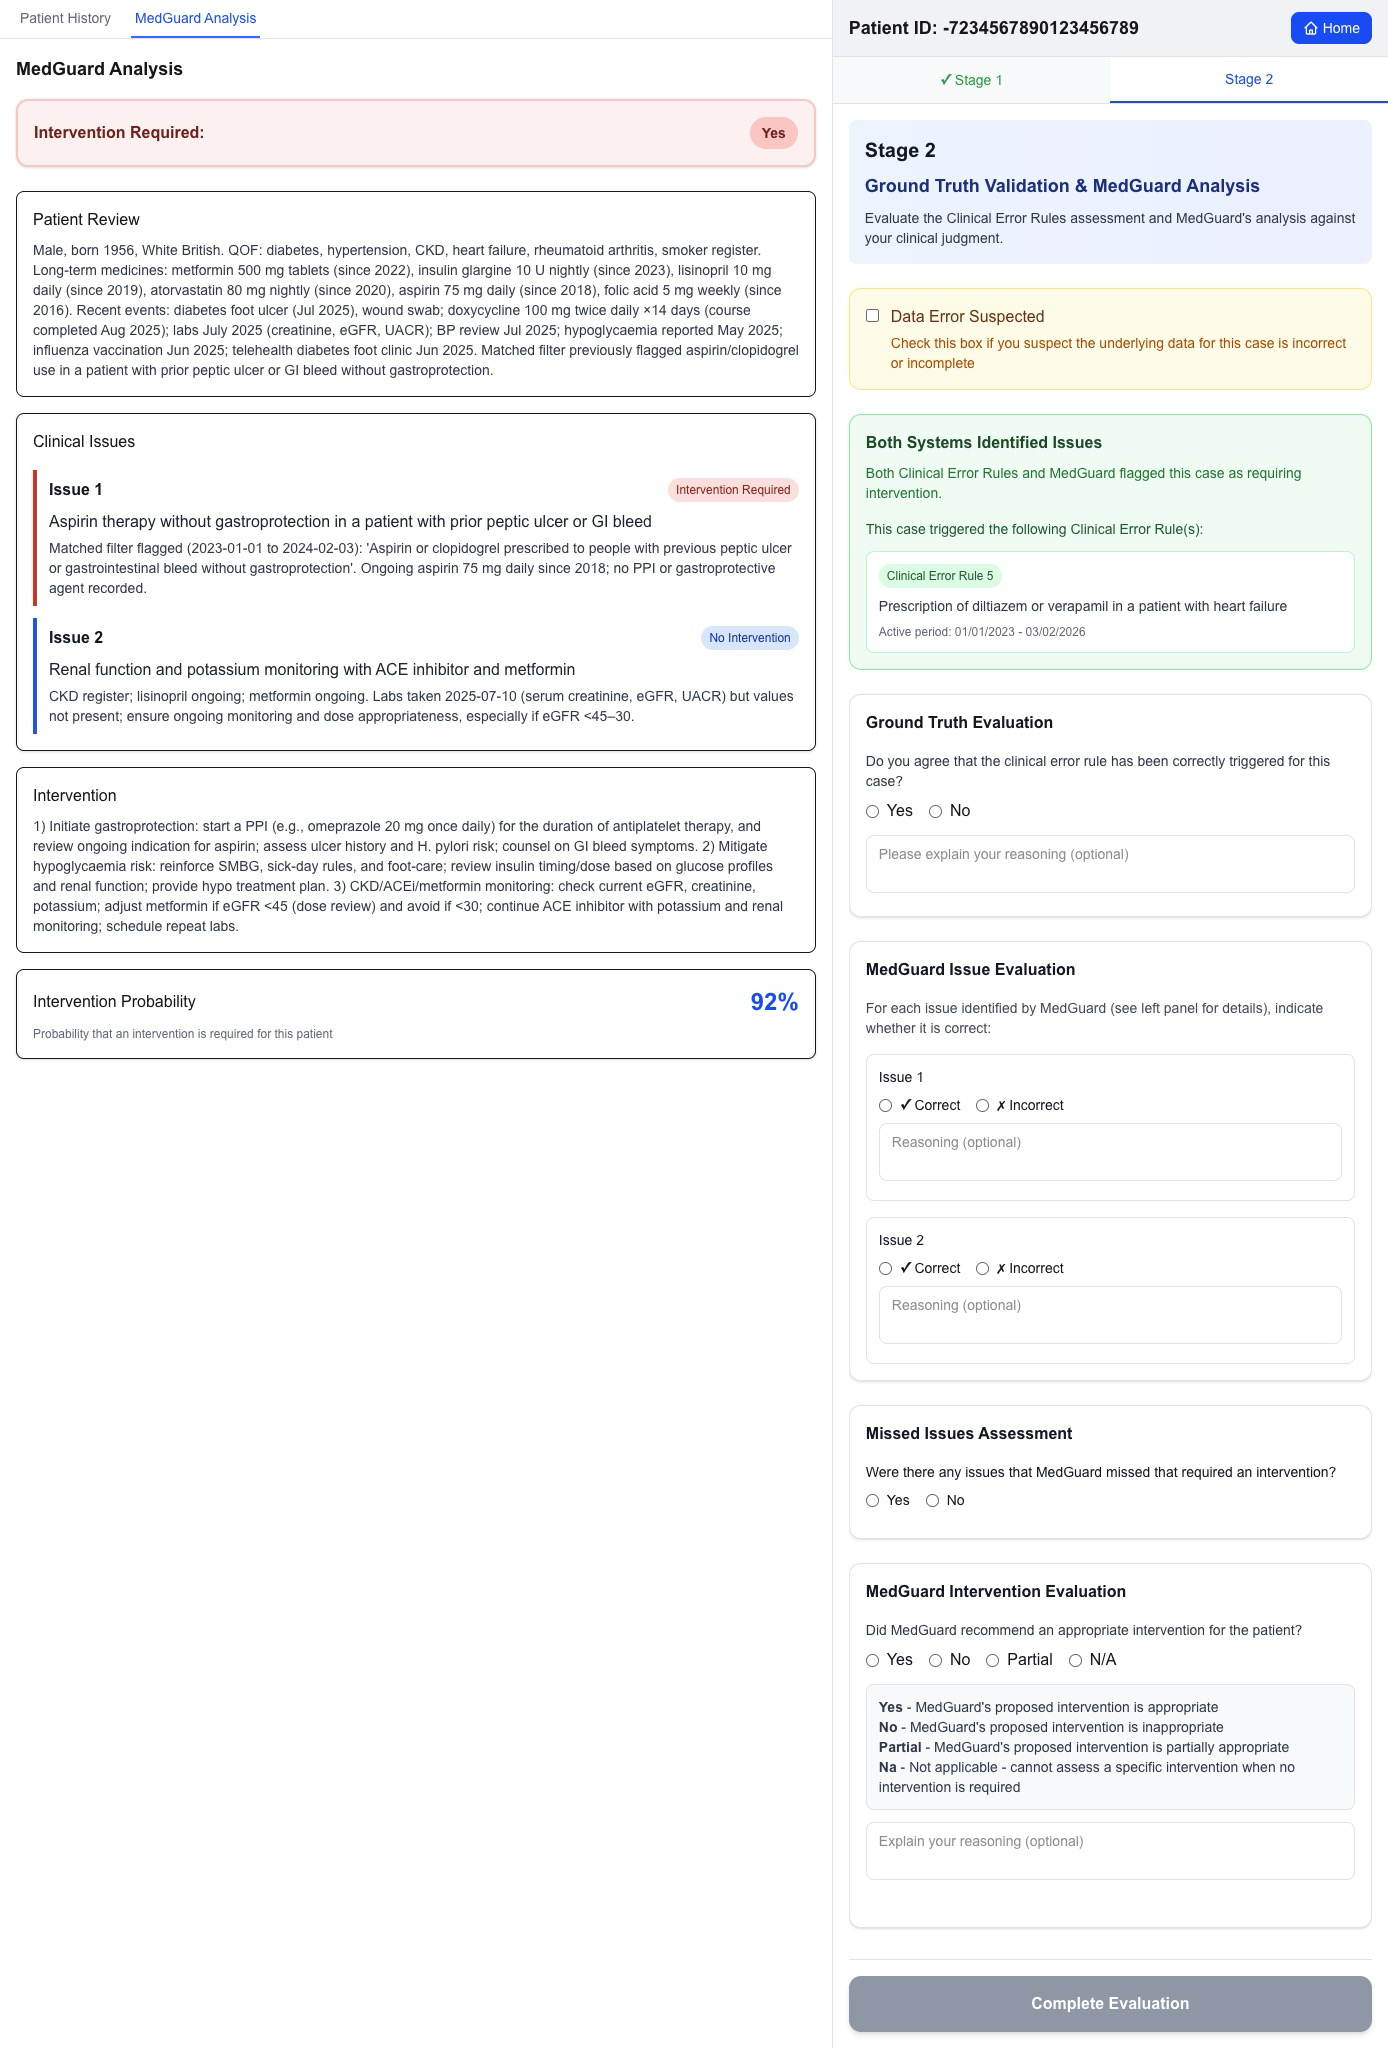
\includegraphics[width=\textwidth]{figures/stage_2_evaluation_app.png}
        \caption{Screen 2: The clinician can look at the structured patient data, and the System's analysis. They then grade the System's issues and interventions.}
        \label{fig:stage_2_evaluation_app}
    \end{subfigure}
    \caption{Clinician Evaluation App}
    \label{fig:evaluation_apps}
\end{figure}